
\chapter{Test phase \#3}\label{ch:test_3}

Le travail effectué pendant le projet est validé dans son ensemble par le test de la phase \#3. Ce test permet de vérifier que tous les éléments développés durant l'entier de la période de réalisation du projet sont à la hauteur de ce qui est attendu et remplissent leur tâche correctement. Il permet également de jauger si la problématique au cœur du projet est en partie solutionnée par le système proposé.

Les éléments développés pour ce test sont les suivants:

\begin{itemize}
\item Ajout de l'acquisition du rythme cardiaque et de la cadence au capteur
\item Gestion et stockage des nouveaux paramètres ajoutés au capteur par la passerelle
\item Finalisation de l'application mobile
\end{itemize}

Le capteur est modifié afin de pouvoir compter les battements du cœur ainsi que l'intervalle de temps afin de permettre le calcul du nombre de battements par minute. De même pour la cadence, l'accéléromètre est interrogé périodiquement pour récupérer les valeurs d'accélération et tenter de détecter les pas. Ces données sont ensuite transmises à la passerelle à l'intérieur des paquets LoRa.
Une boîte permettant d'insérer le capteur ainsi que tous les autres éléments (l’accumulateur, le module rythme cardiaque, l'antenne GPS et LoRa) est construite puis imprimée grâce à une imprimante 3D. Une sangle élastique permet de fixer le capteur au bras du cobaye.

La configuration de la passerelle est modifiée pour automatiquement lancer l'exécution du packet forwarder et du serveur d'application lors de son lancement, ce qui permet de ne pas devoir effectuer d'autres opérations que de la mettre sous tension pour qu'elle soit opérationnelle.
Le traitement des nouvelles données reçues dans les paquets est implémenté dans le code du serveur d'application de la passerelle. Une fois les données extraites, le tout est sauvegardé dans la base de données.

Pour ce test, le gros du travail est centré autour de l'application mobile. Toutes les fonctions de gestion de course sont implémentées, comme la création de nouvelles courses ainsi que l'inscription des coureurs. Les modes de visualisation de course est complété avec l'affichage de toutes les nouvelles informations à disposition, le rythme cardiaque et la cadence, mais également les informations qui sont calculées à partir des données reçues, la distance parcourue, la vitesse moyenne et le temps de course. L'interface graphique est finalisée afin de pouvoir montrer toutes les informations au spectateur et une phase de affinage est effectuée pour rendre le tout cohérent et agréable à l'utilisation.

Le code utilisé durant ce test correspond au tag de la version v1.0 sur git.

\section{Scénarios}

Une nouvelle fois, le système est mis à l'utilisation dans un cadre permettant un test en conditions réelles. Avant le démarrage du test, la course est créée directement depuis l'application mobile, alors que pour les tests des phases précédentes les courses étaient créées manuellement dans la base. L'inscription de la coureuse est également faite dans l'interface de l'application, enfin la course est démarrée.

Au terme de la création de la course, deux tests sont effectués.

Le premier test consiste à mettre le capteur sous tension grâce à l'accumulateur puis d'attendre la synchronisation GPS. Lorsque le module GPS est prêt à acquérir des positions avec assez de précision, la coureuse s'élance sur la piste afin de faire quelques tours de la piste d'athlétisme permettant ainsi de vérifier que tout fonctionne bien.

Le deuxième test consiste à voir comment le capteur se comporte lorsqu'il n'a plus la vue directe sur la passerelle mais qu'elle est obstruée par un obstacle comme un bâtiment par exemple.

Durant les deux tests les parcours ont également été enregistrés  avec une montre GPS sur la plateforme Strava qui permet d'enregistrer ses courses. Cela permettra de comparer les résultats de chaque application et vérifier qu'aucune grosse erreur n'existe.

\section{Résultats}

Les deux tests ont pu être menés à bien le 22 Septembre 2018 au stade d'athlétisme de Colombier.

\subsection{Test de validation du système}

Pendant ce test, la coureuse a fait 3 fois le tour de l'anneau d'athlétisme, ce qui a permis de vérifier que les paramètres rapportés par l'application mobile étaient vraisemblables.

Afin de pouvoir comparer les résultats obtenues par le système, la course enregistrée sur la plateforme Strava peut être consultée à l'adresse \url{https://www.strava.com/activities/1858813564}.

Sur la figure \ref{fig:test_3}, on peut voir que très rapidement des valeurs de rythme cardiaque et de cadence apparaissent sur l'interface de l'application mobile. En comparant les valeurs de rythme cardiaque avec celle de la plateforme Strava, elles semblent être conformes à la réalité. Par contre, on peut remarquer que les valeurs de cadences sont totalement fausses, elles devraient être aux alentours de 160-170 pas par minute au lieu de 11-48.

En ce qui concerne les positions GPS, comme durant le test phase \#2, on peut voir que la précision est très bonne et que les positions sont conformes au tracé effectué durant le test. On remarque que, comme montré dans la figure \ref{fig:test_3_track3}, après 2 tours de piste, c'est à dire 800 m de course, l'application montre une distance de 0.79 km ce qui est très proche de la réalité.

Au terme de l'exercice, on peut voir les valeurs totales enregistrée par l'application sur la figure \ref{fig:test_3_track4}. Une comparaison entre les résultats obtenus et ceux de la plateforme Strava est disponible dans la table \ref{tab:comp_results}. On peut voir que les résultats des deux applications sont très proches, ce qui permet d’affirmer que la précision des données calculées et acquises par le système est bonne. Si l’on prend en considération qu'une montre GPS enregistre beaucoup plus de positions que le capteur qui n'en enregistre qu'une toutes les 15 secondes, on peut comprendre l'erreur qu'il y a entre les deux systèmes. En effet, le fait d'acquérir beaucoup plus de points permet d'avoir un calcul de la distance totale plus proche de la réalité, car elle est calculée en tirant une droite entre deux point du tracé.

\begin{table}[htb]
\caption{Comparaison des résultats}
\label{tab:comp_results}
\centering
\begin{tabular}{ l l l l }
\toprule
Plateform & Distance & Temps & Vitesse Moyenne  \\
\midrule
Strava & 1.2 km & 6.08 min & 5.07 min/km \\
TB & 1.1 km & 6.15 min & 5.4 min/km \\
\bottomrule 
\end{tabular}
\end{table}

\begin{figure}[tb]
\centering
\begin{subfigure}{0.7\textwidth}
  \centering
  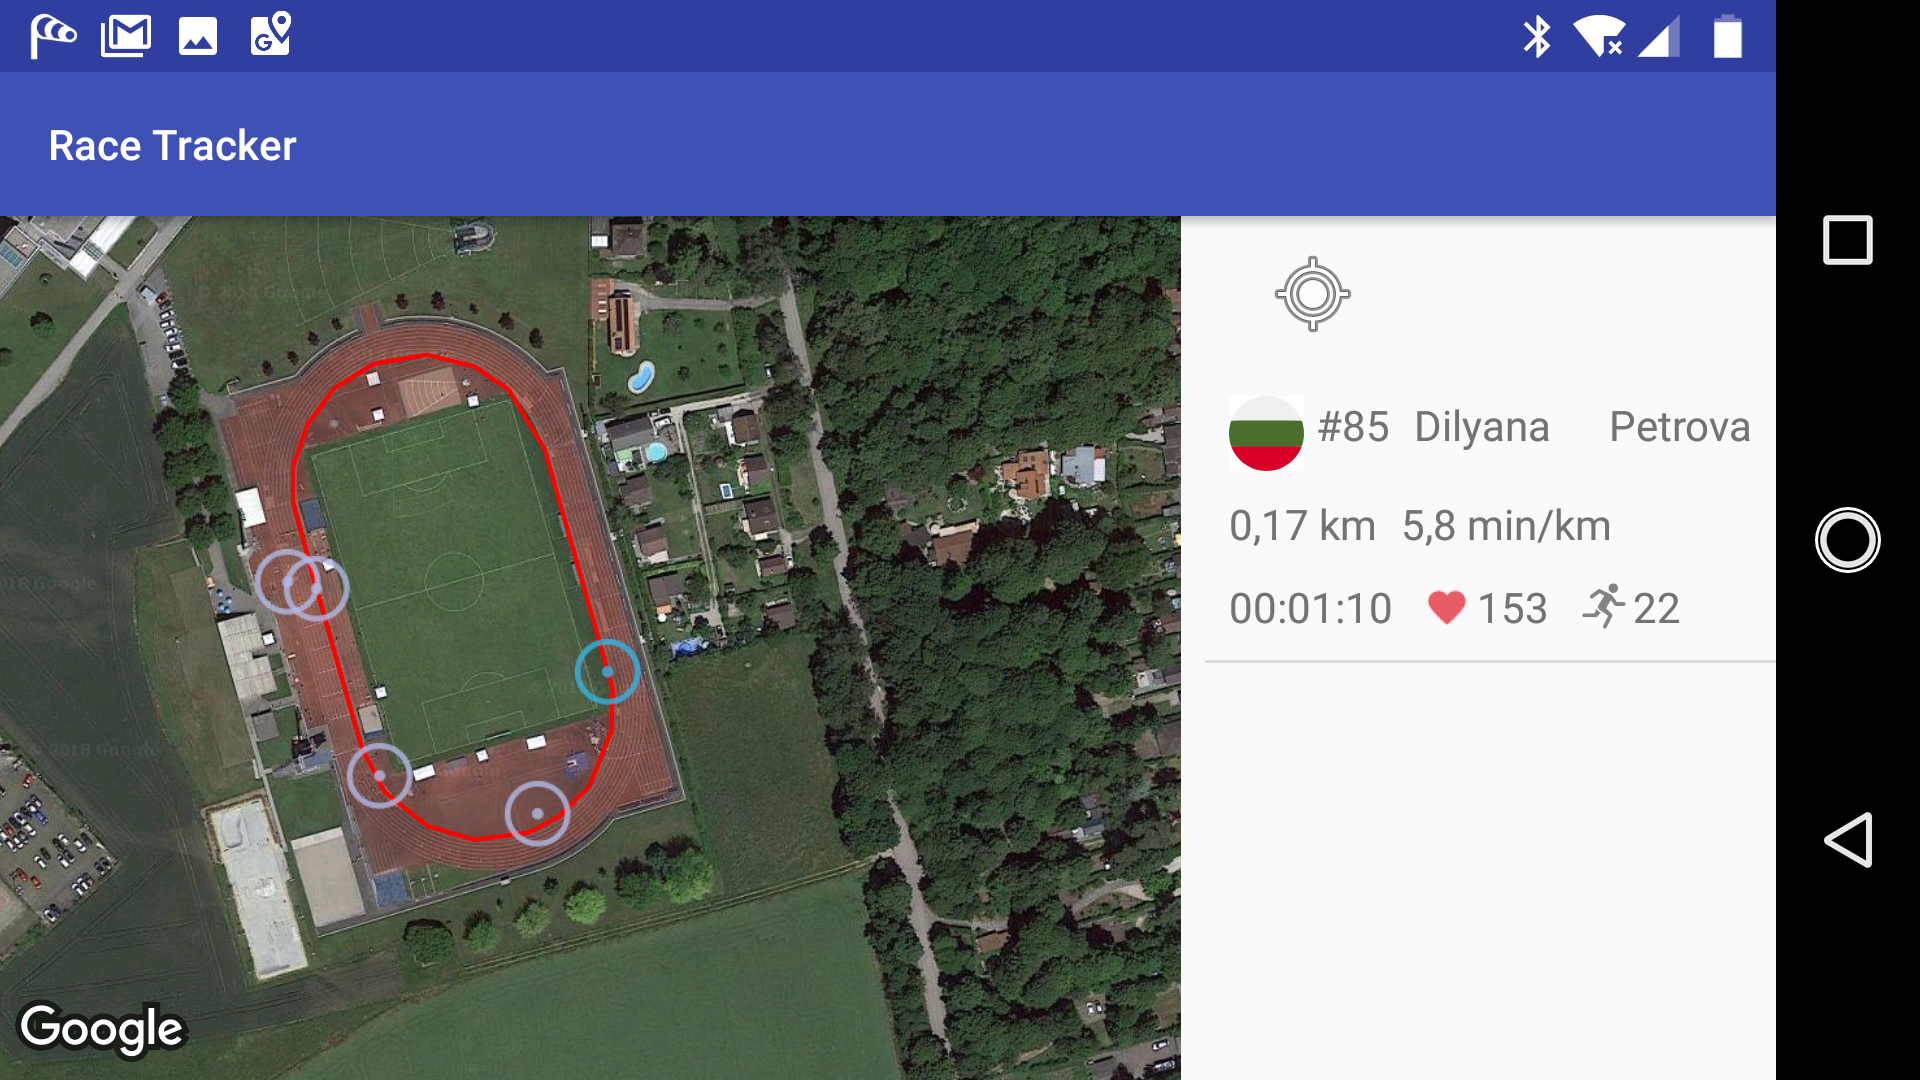
\includegraphics[width=0.9\linewidth]{test_3_track1.png}
  \caption{Test \#3 - Image \#1}
  \label{fig:test_3_track1}
\end{subfigure}%

\begin{subfigure}{0.7\textwidth}
  \centering
  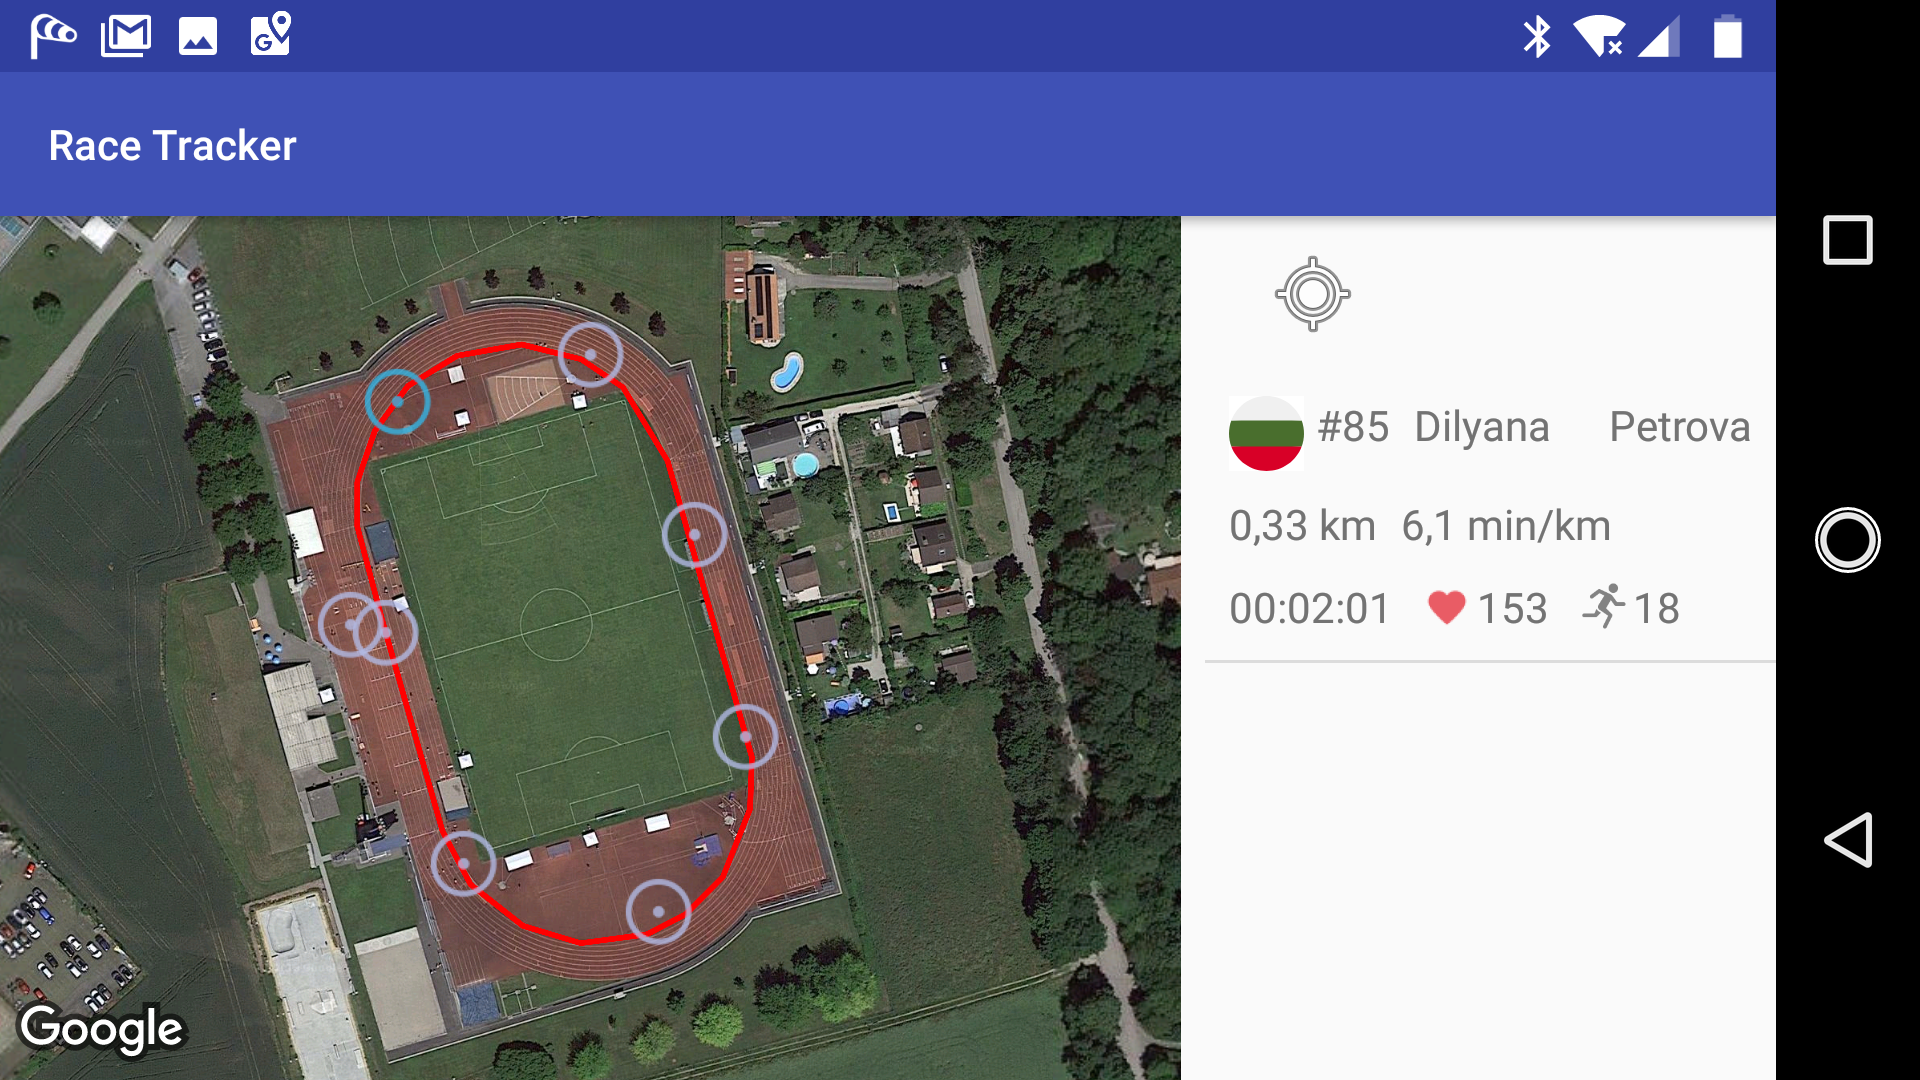
\includegraphics[width=0.9\linewidth]{test_3_track2.png}
  \caption{Test \#23- Image \#2}
  \label{fig:test_3_track2}
\end{subfigure}

\begin{subfigure}{0.7\textwidth}
  \centering
  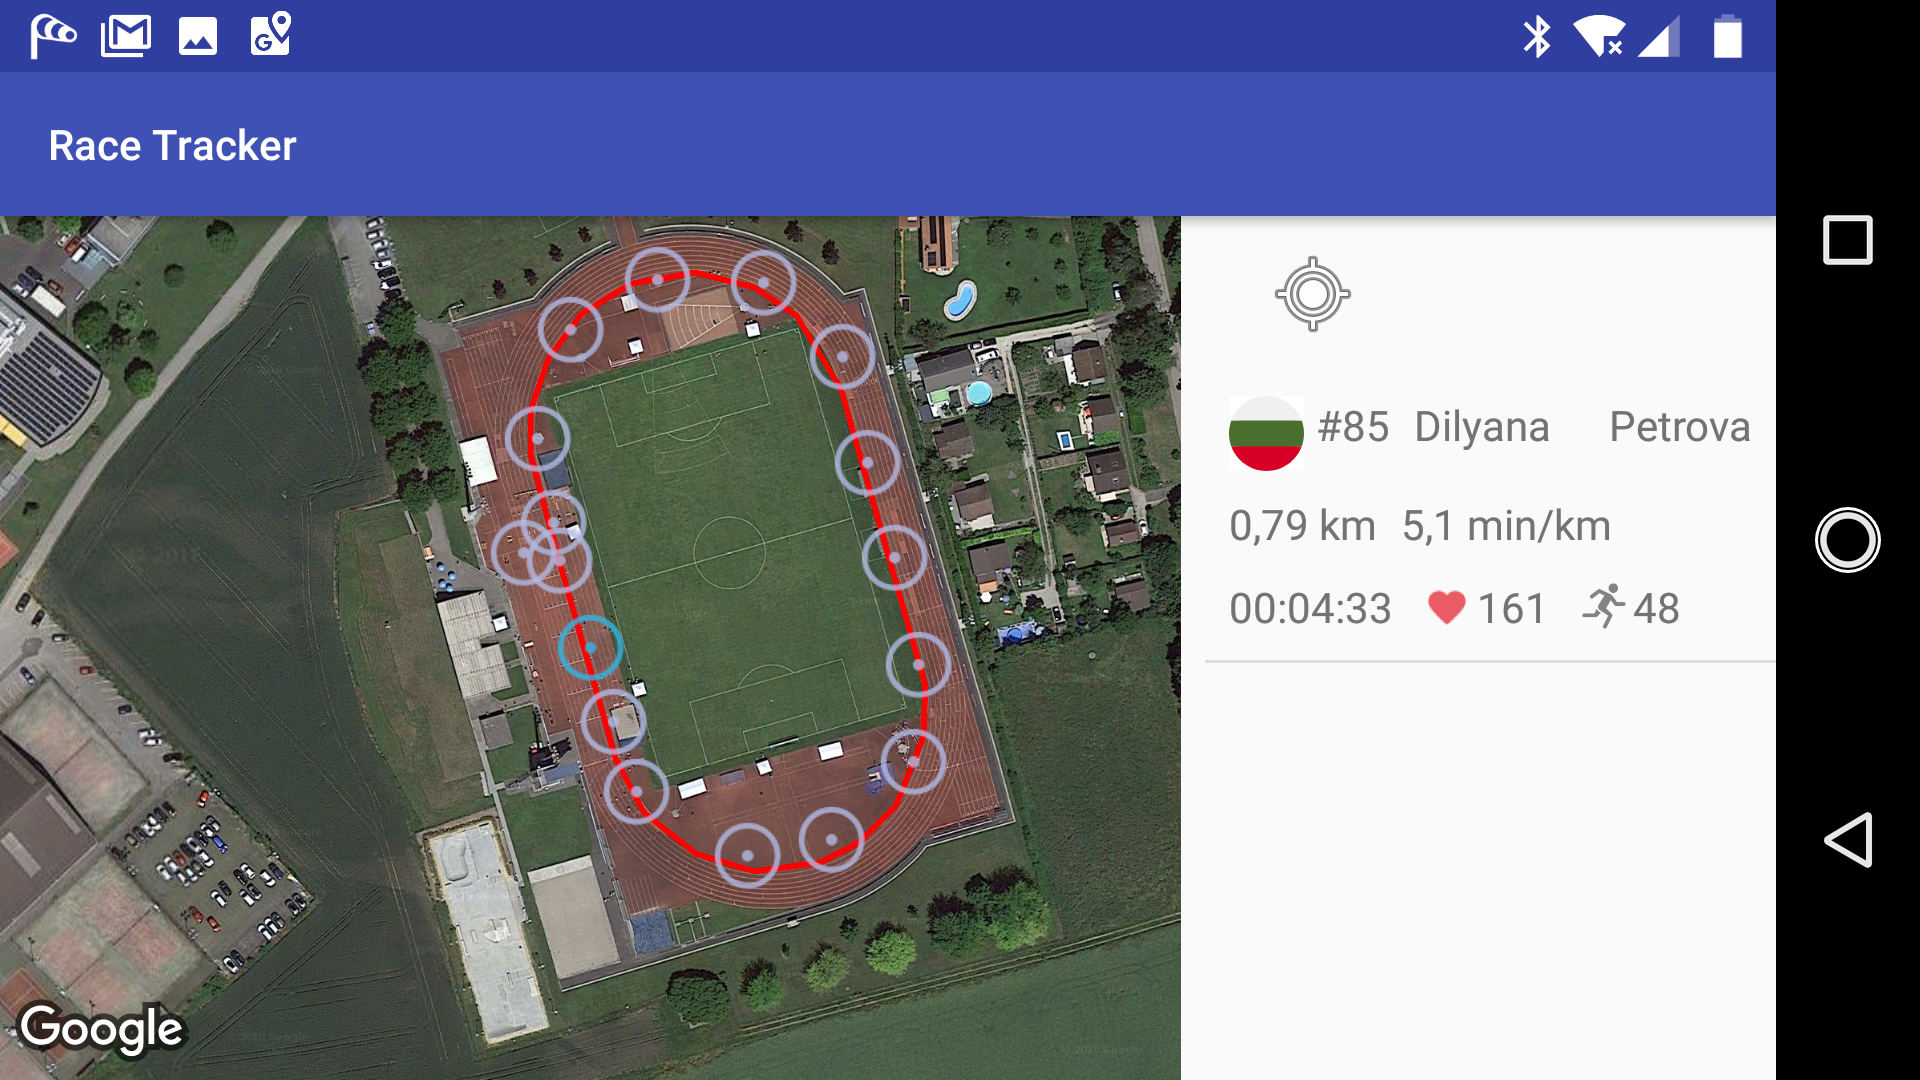
\includegraphics[width=0.9\linewidth]{test_3_track3.png}
  \caption{Test \#3 - Image \#3}
  \label{fig:test_3_track3}
\end{subfigure}%

\begin{subfigure}{0.7\textwidth}
  \centering
  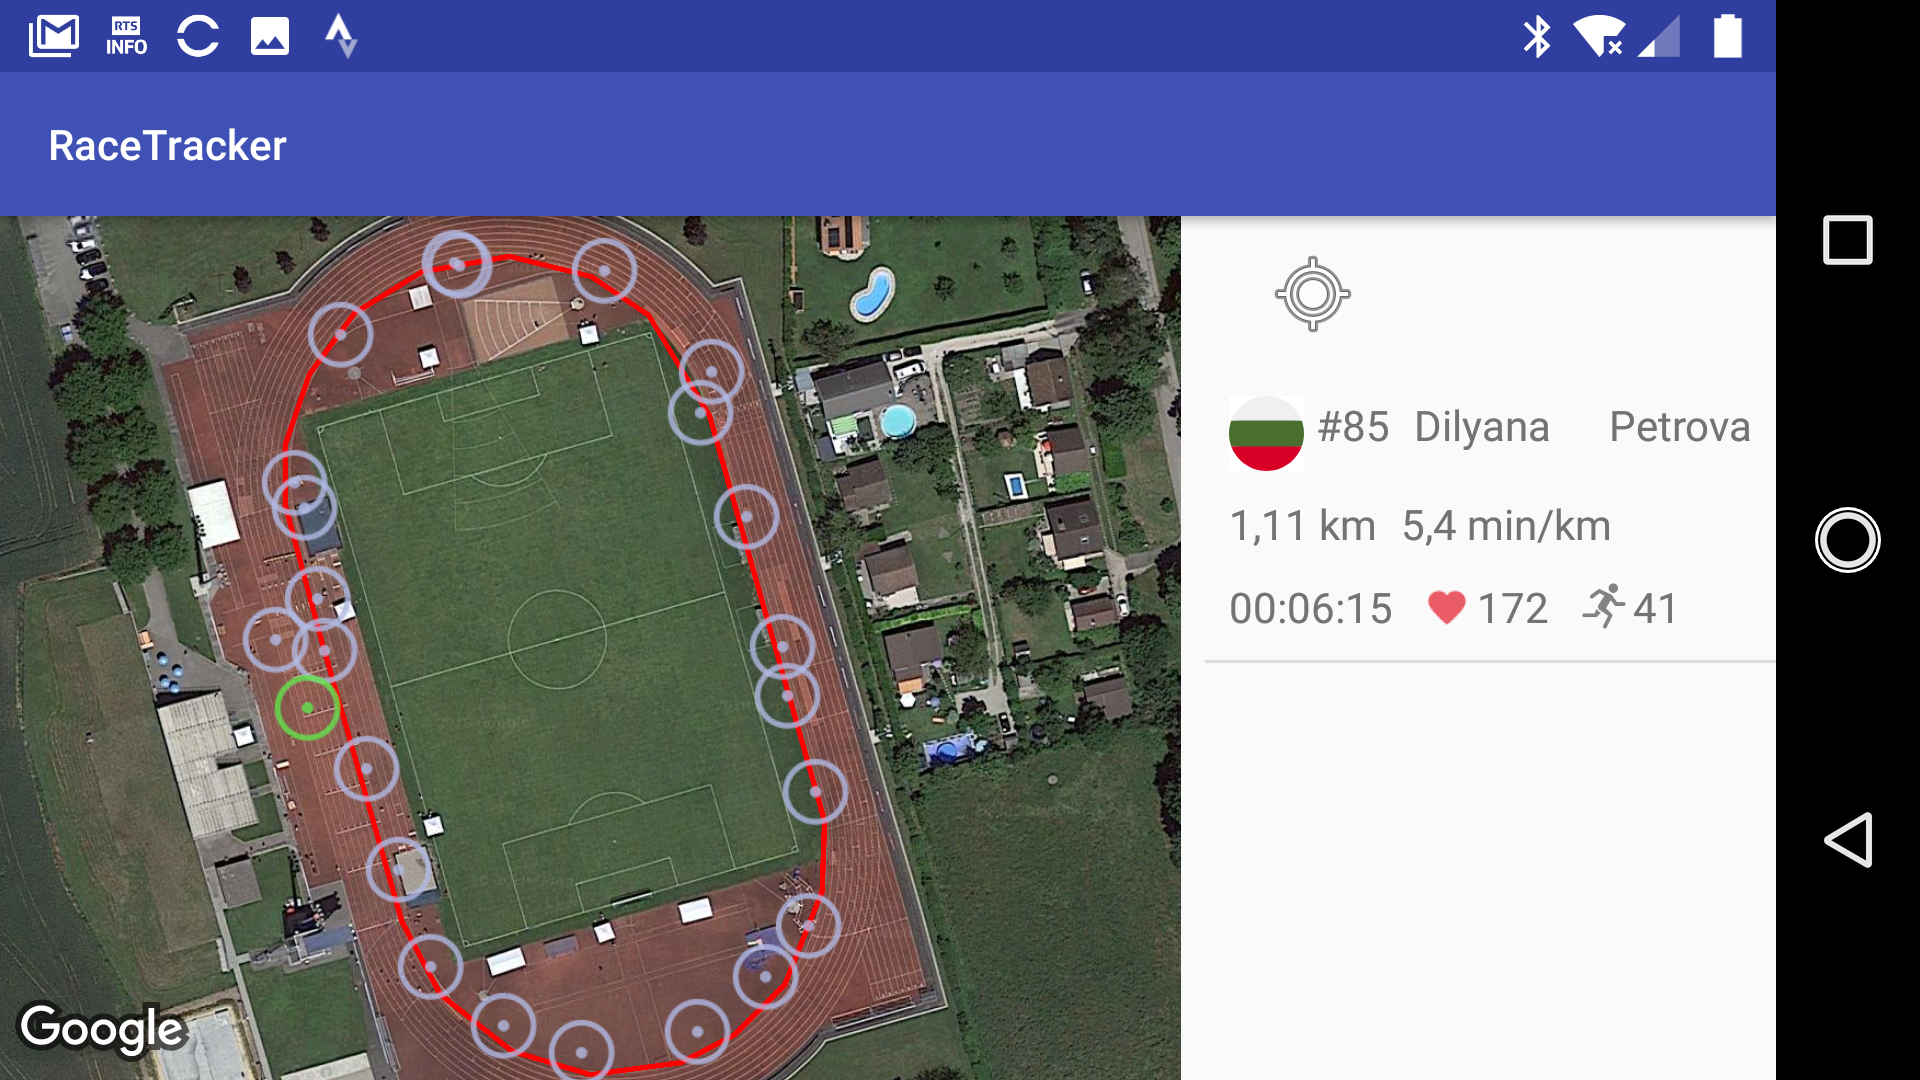
\includegraphics[width=0.9\linewidth]{test_3_track4.png}
  \caption{Test \#23- Image \#4}
  \label{fig:test_3_track4}
\end{subfigure}
\caption{Visualisation de l'application mobile pour le test 3}
\label{fig:test_3}
\end{figure}

\subsection{Test obstruction passerelle}

Le test d'obstruction consiste à courir dans un emplacement où la passerelle et le capteur ne sont plus en vue l'un de l'autre. Le but étant de vérifier si dans ces conditions les positions étaient en mesure d'atteindre la passerelle.

Il est possible de consulter la course de comparaison à l'adresse \url{https://www.strava.com/activities/1858813761}.

La figure \ref{fig:test_3_obstru} montre en rouge le tracé du chemin emprunté par la coureuse. On remarque que les premiers points sont bien reçus puis très rapidement la trace du capteur est perdue. Cet exercice permet de constater que malgré les arguments marketing qui promettent d'arriver à atteindre des distances de communication de plusieurs kilomètre en ville, un simple bâtiment peut rapidement empêcher toute communication de se faire.

\begin{figure}[htb]
\centering 
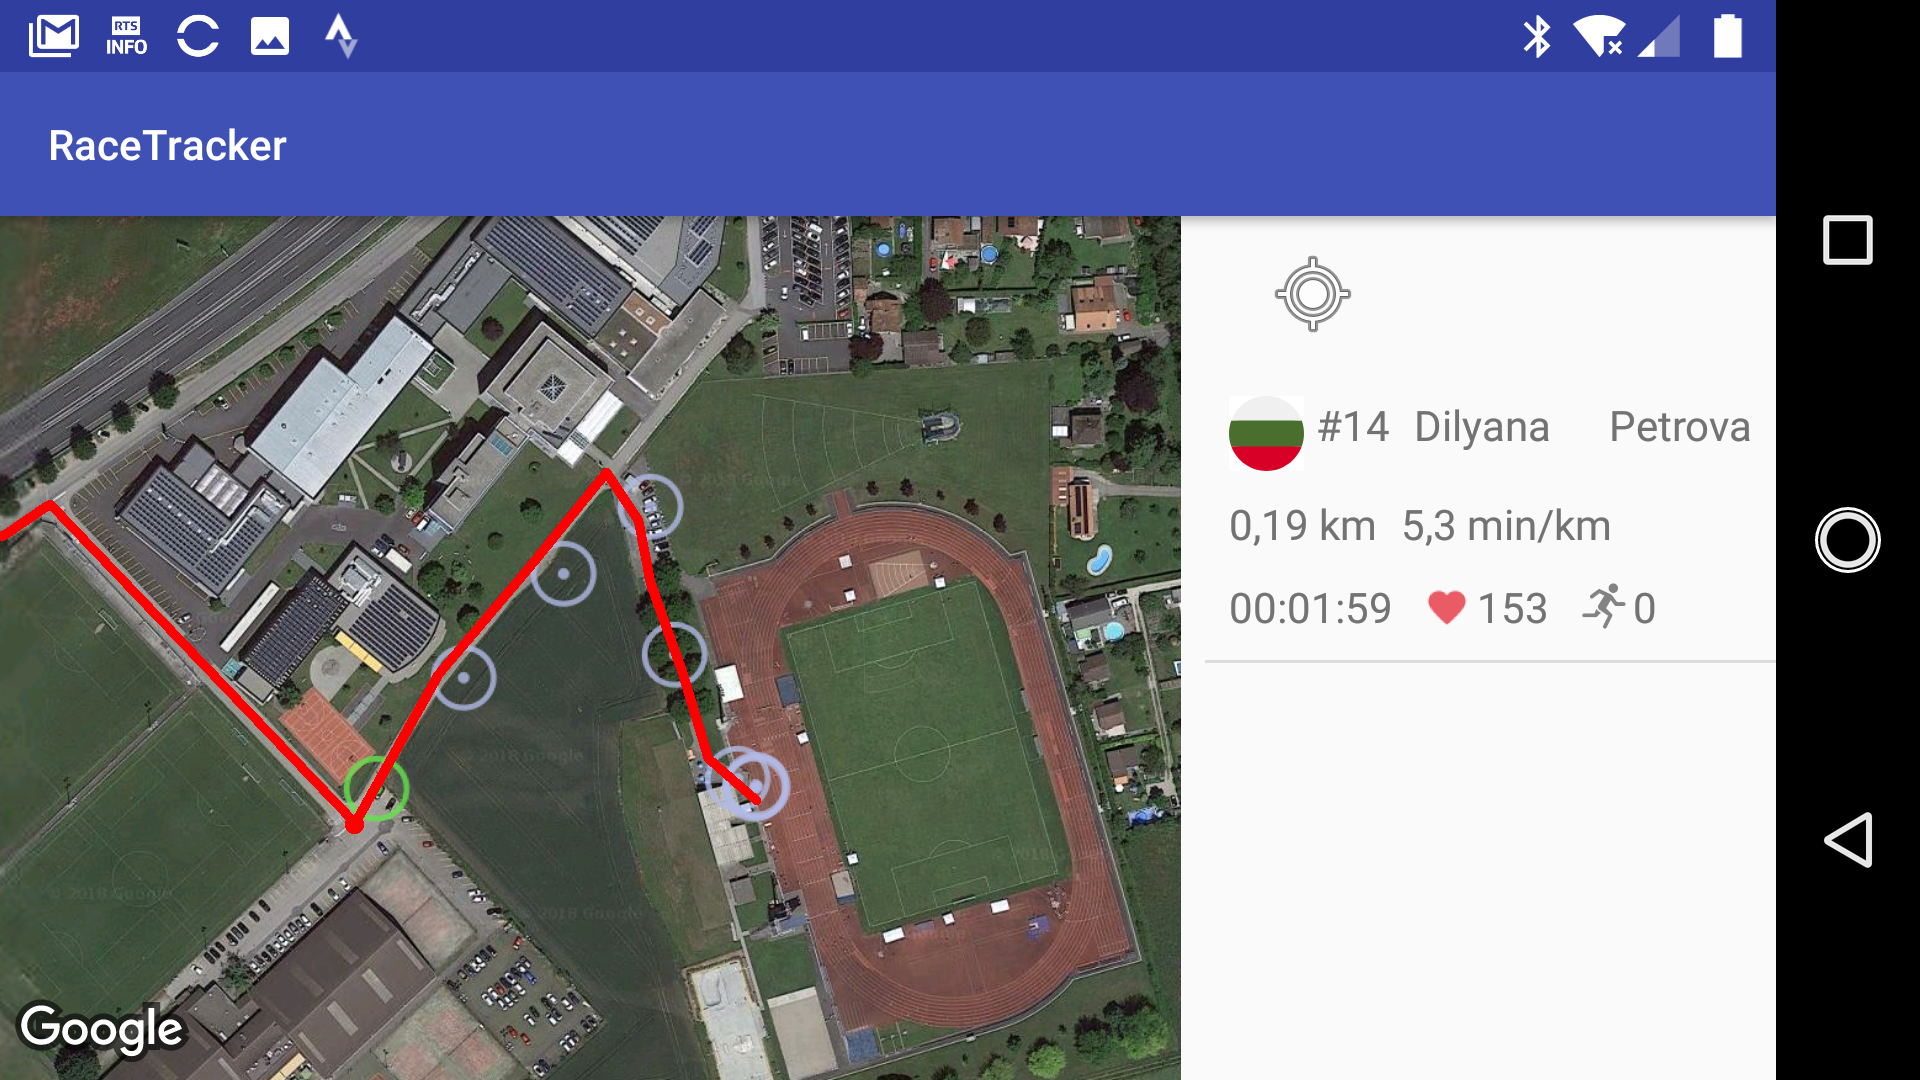
\includegraphics[width=0.8\columnwidth]{test_3_obstruction_1.png} 
\caption{Résultats du test d'obstruction}
\label{fig:test_3_obstru}
\end{figure}

\section{Conclusions}

Le test de la phase \#3 a permis de valider le fonctionnement du système dans son ensemble. Premier point positif, on peut déjà dire que malgré quelques problèmes le concept du système fonctionne bien, les positions GPS sont mises à jour correctement et elles sont justes. Le rythme cardiaque, la distance totale ainsi que la vitesse moyenne montrent des valeurs proche de la réalité ce qui permet d'affirmer que le gros du système est à la hauteur des attentes.

Pour ce qui est de la cadence, même si on voit que des valeurs sont remontées à l'application, ce qui est encourageant, on remarque que les valeurs elles-mêmes sont totalement fausses, ceci étant dû au fait que les pas ne sont pas du tout détectés avec assez de précision, ce qui fait que le compte est faux et donc la cadence également. L'algorithme de détection des pas requiert plus de travail afin de pouvoir calculer une cadence correcte.

Le test a également mis en lumière que la communication LoRa semble être plus sensible qu'escompté aux obstructions entre l'émetteur et le récepteur. Cet aspect demande plus de tests afin de pouvoir dire précisément les effets de l'obstruction, cependant cet élément peut devenir problématique pour le système et son utilisation. La seule solution qui pourrait permettre de pallier à ce problème serait l'utilisation d'un grand nombre de passerelles afin d'assurer que le capteur aie toujours la vue sur une d'entre elles afin de pouvoir transmettre les informations.

Dans l'ensemble le test de la phase \#3 est un succès. Même si les résultats ne sont pas entièrement parfaits, le gros du système fonctionne bien et l'utilisation de l'application mobile donne la satisfaction attendue.